\documentclass{ctexart}
\usepackage{tikz}
\usetikzlibrary{trees}
\tikzset{box/.style={rectangle ,rounded corners=5pt, draw}}
\begin{document}
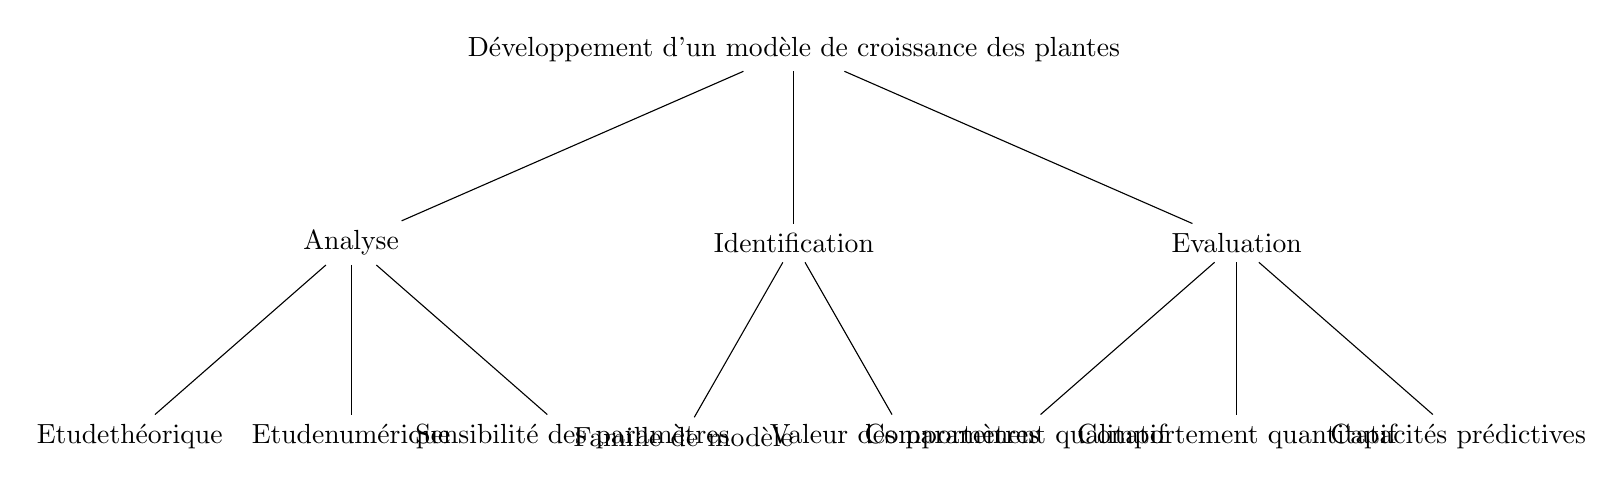
\begin{tikzpicture}[level distance=70pt, sibling distance=5pt]
  
\tikzstyle{level 1}=[sibling distance=160pt]
\tikzstyle{level 2}=[sibling distance=80pt]
\tikzstyle{level 3}=[sibling distance=200pt]
%\tikzstyle{level 4}=[sibling distance=50pt]
%\tikzstyle{level 5}=[sibling distance=80pt]
%\tikzstyle{level 6}=[sibling distance=50pt]
%\tikzstyle{level 7}=[sibling distance=80pt]
%\tikzstyle{level 8}=[sibling distance=50pt]
%\tikzstyle{level 9}=[sibling distance=80pt]

\node{Développement d’un modèle de croissance des plantes}
  child { node {Analyse}
    child { node {{Etude\\ théorique}} }
    child { node {Etude \\ numérique}}
    child { node {Sensibilité des paramètres}}
    }
    child { node {Identification}
    child { node {{Famille de modèle}} }
    child { node {Valeur des paramètres}}
    }
    child { node {Evaluation}
    child { node {{Comportement qualitatif} }}
    child { node {Comportement quantitatif}}
    child { node {Capacités prédictives}}
    };
\end{tikzpicture} 
\end{document}